\documentclass{article}

\usepackage[hidelinks]{hyperref}

\usepackage{tikz}
\usetikzlibrary{matrix,chains,positioning,decorations.pathreplacing,arrows}

\usepackage[color=cyan]{todonotes}

\usepackage{minted}
\usemintedstyle{colorful}

\addtolength{\oddsidemargin}{-.875in}
\addtolength{\evensidemargin}{-.875in}
\addtolength{\textwidth}{1.75in}

\addtolength{\topmargin}{-.875in}
\addtolength{\textheight}{1.75in}

\bibliographystyle{plain}

\begin{document}

\title{An Application of Deep Neural Networks to Programming Language Classification}
\author{Erik Boesen, Candidate gsg256}
\maketitle

\begin{abstract}
We assess the extent to which artificial neural networks can be used to distinguish between programming languages. We use an artificial deep neural network to achieve a success rate of \todo{Insert success rate} at distinguishing between 8 different programming languages following supervised training.
\end{abstract}

\section{Introduction}
In this research we seek to develop and implement a neural network which differentiates between the world's 10 most commonly used programming languages according to the TIOBE Index \cite{tiobe}, a popular index tracking the prevalence of programming languages as measured by search engine queries. The top 10 languages according to the May 2018 iteration of the Index are Java, C, C++, Python, C\#, Visual Basic .NET, PHP, JavaScript, SQL, and Ruby. The learning techniques used are generalizable to any selection of languages.

In this paper, we explain the rudiments of neural networking techniques used, and give implementation examples using C++ (explaining and keeping to a minimum any idiomatic syntax).

\subsection{A general overview of neural networks}
\subsubsection{Why use a Neural Network?}
Neural Networks are a common technique used in the burgeoning field of machine learning. Machine learning techniques are useful when a large and diverse set of data must be processed (often entailing categorization), but when writing explicit code to make distinctions between data points would be impractical. For example, when identifying objects in an image, as in \cite{hinton12}, it would be nearly impossible to write a procedure to directly read image data and distinguish between many images. Though there exist simpler machine learning techniques, such as the K Nearest Neighbors algorithm, these strategies have trouble making decisions in so many dimensions with such a complex output vector as demonstrated in \cite{knnic}. Though the concept of a neural network was first proposed in 1958 \cite{rosenblatt58}, the concept has recently experienced a resurgence of popularity. Machine learning techniques based on neural networks including deep learning \cite{mitdeeplearning} and recurrent neural networks \cite{recurrentsurvey} have recently been applied to diverse problems, including achieving victory over a human in the age-old game of Go \cite{go1}\cite{go2}, differentiating between multiple thouands of different image classes \cite{hinton12}, and even recognizing verbal speech \cite{rnnspoken}.

\subsubsection{Structure}
Neural Networks make tasks like the aforementioned easier by taking cues from neurobiology and simulating how a real brain makes decisions. In the brains of humans and other animals, many neurons are joined together. These neurons themselves simply take electrical input, adjust it, and pass it along to the next neuron. Biological brains readjust the behavior of their individual constituent neurons, and in doing so are able to perform the process of learning.

Though this is a gross oversimplification of the actual biological processes of learning and neuroplasticity, it may be a helpful metaphor to understand the function of an artificial neural network: the technique is remarkably similar, as you will see.

The process performed by each neuron during training is relatively simple and is thus easier to think about independently. First, the neuron sums the output values $\xi$ of all neurons in the previous layer, including a static bias neuron, multiplying each value by calculated weights $\omega$ which are adjusted while the network is trained. The resulting values then pass through an activation function, which brings the output into a regular range such as $(0, 1)$ or $(-1, 1)$. There exist many different activation functions, however, in this investigation we use the common $\sigma$ ("sigmoid") function, which limits our neuron's output to $(0, 1)$:
$$\sigma(x)=\frac{1}{1+e^{-x}}$$
Hence, you may think of the neuron output $\mathcal{O}$ thus:
$$\mathcal{O}=\sigma(\sum_n[w_{n}\xi_{n}])$$
After the activation function is applied, the returned value is given as the neuron's output, and the process is repeated, using that output as the input for successive neurons. A single neuron, hence, might be visualized as follows:

\begin{center}
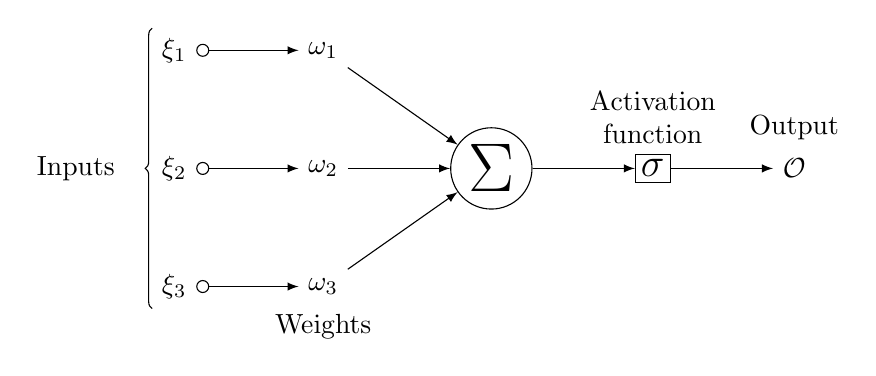
\begin{tikzpicture}[
init/.style={draw, circle, inner sep=2pt, font=\Huge, join = by -latex},
squa/.style={draw, inner sep=2pt, font=\Large, join = by -latex},
start chain=2,node distance=13mm
]
\node[on chain=2] (x2) {$\xi_2$};
\node[on chain=2, join=by o-latex] {$\omega_2$};
\node[on chain=2, init] (sigma) {$\displaystyle\Sigma$};
\node[on chain=2, squa,label=above:{\parbox{2cm}{\centering Activation \\ function}}] {$\sigma$};
\node[on chain=2, label=above:Output,join=by -latex] {$\mathcal{O}$};
\begin{scope}[start chain=1]
  \node[on chain=1] at (0,1.5cm) (x1) {$\xi_1$};
  \node[on chain=1, join=by o-latex] (w1) {$\omega_1$};
\end{scope}
\begin{scope}[start chain=3]
  \node[on chain=3] at (0,-1.5cm) (x3) {$\xi_3$};
  \node[on chain=3, label=below:Weights, join=by o-latex] (w3) {$\omega_3$};
\end{scope}

\draw[-latex] (w1) -- (sigma);
\draw[-latex] (w3) -- (sigma);

\draw[decorate,decoration={brace,mirror}] (x1.north west) -- node[left=10pt] {Inputs} (x3.south west);
\end{tikzpicture}
\end{center}

Understanding now the basic logic behind individual neurons, we turn to the the architecture of a full neural network. In the most basic format, known frequently as a ``feed forward'' network, a neural network contains three types of layers, each of which is a vector of neurons, each taking input from every neuron in the previous layer without interacting with the rest of the layer.
\begin{itemize}
\item{The first layer is the \textbf{input layer}. Input data is fed directly into this layer, and the number of neurons typically is the same as the number of input values.}
\item{Following the input layer comes at least one \textbf{hidden layer} (more than one in deep neural networks). The output values of the neurons in these layers are not necessarily returned to a user, rather, they are passed on to the following layer, which can be the output layer or another hidden layer.}
\item{Neurons in the \textbf{output layer} return the output of the neural network. Note that traditionally, the activation function is implemented here as well, so basic feed forward networks are generally capable only of outputting a value in the range of the chosen activation function.}
\end{itemize}

\begin{center}
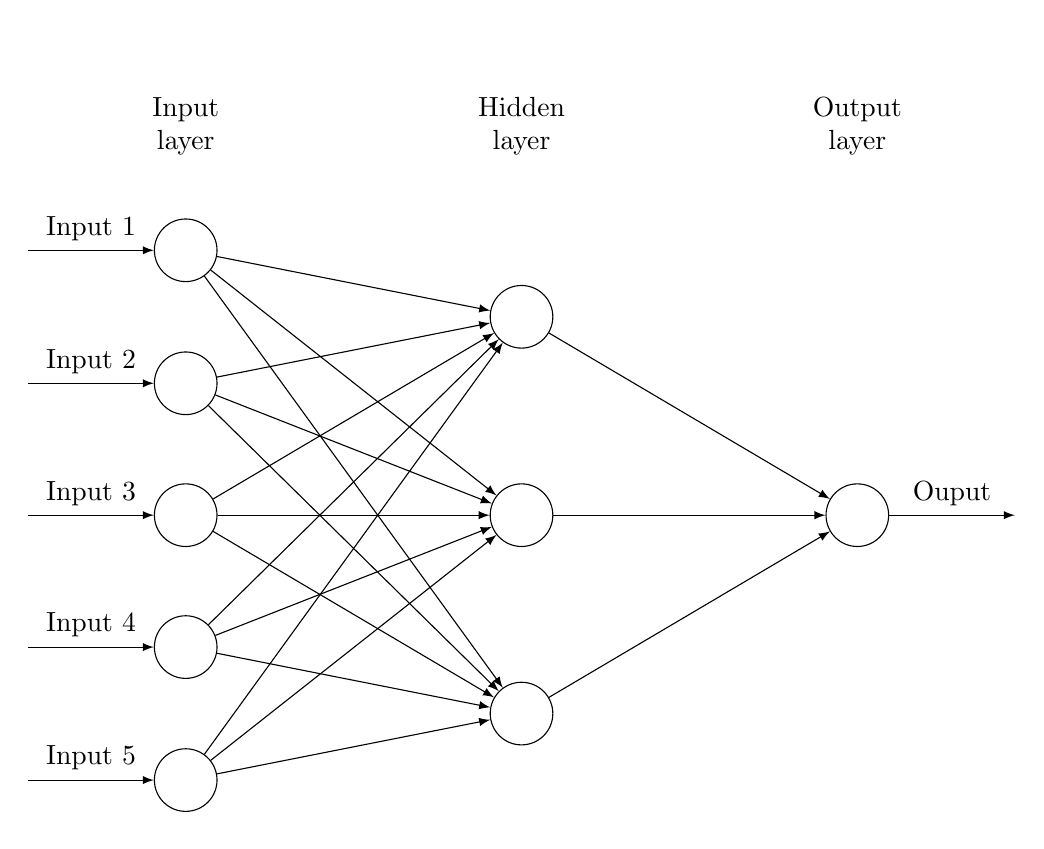
\begin{tikzpicture}[
plain/.style={draw=none, fill=none},
net/.style={matrix of nodes, nodes={draw, circle, inner sep=8pt}, nodes in empty cells, column sep=2cm, row sep=1pt}, >=latex
]
\matrix[net] (mat)
{
|[plain]| \parbox{1.3cm}{\centering Input\\layer} & |[plain]| \parbox{1.3cm}{\centering Hidden\\layer} & |[plain]| \parbox{1.3cm}{\centering Output\\layer} \\
& |[plain]| \\
|[plain]| & \\
& |[plain]| \\
  |[plain]| & |[plain]| \\
& & \\
  |[plain]| & |[plain]| \\
& |[plain]| \\
  |[plain]| & \\
& |[plain]| \\    };
\foreach \ai [count=\mi ]in {2,4,...,10}
  \draw[<-] (mat-\ai-1) -- node[above] {Input \mi} +(-2cm,0);
\foreach \ai in {2,4,...,10}
{\foreach \aii in {3,6,9}
  \draw[->] (mat-\ai-1) -- (mat-\aii-2);
}
\foreach \ai in {3,6,9}
  \draw[->] (mat-\ai-2) -- (mat-6-3);
\draw[->] (mat-6-3) -- node[above] {Ouput} +(2cm,0);
\end{tikzpicture}
\end{center}

\subsection{Backpropogation}
A central component of neural network training is the process of backpropogation. In very general terms, backpropogation is the process of determining the ``error'' of the network, or the difference between outputs the network delivers and desired outputs, during training, and subsequently going backward through the network and adjusting neuron weights and biases accordingly.

To calculate error for an individual output neuron, the process is quite simple: we need only to find the difference between the neuron output $\omega_n$ and the known target value $t_n$.
$$E_n=t_n-\mathcal{O}_n$$
We can then expand this function to find the total error of the network during one epoch (training iteration) as follows. This equation is frequently referred to as the ``cost function.'' \cite{mediummlbasics}
$$C=\frac{1}{2}\sum_n(t_n-\mathcal{O}_n)^2$$
In the context of popular neuroscience (originally in \cite{neuronsfire}), the adage is frequently repeated that ``neurons which fire together, wire together.'' This concept persists in artificial neural networks as well as natural. Through backpropogation, we recursively readjust weights proportionally to their influence on output so as to achieve a more accurate result.

The essence of backpropogation lies in calculating $\frac{\partial{C}}{\partial{\omega}}$ of all weights, or, concretely, the extent to which shifts in each synapse weight affect the final amount of error. Let us first derive the backpropogation algorithm \cite{derivebackprop}. Given the sigmoid activation function:
$$\sigma(x)=\frac{1}{1+e^-x}$$
We can derive:
$$\sigma'(x)=\frac{e^-x}{(1+e^-x)^2}=\frac{(1+e^-x)-1}{(1+e^-x)^2}=\frac{1+e^-x}{(1+e^-x)^2}-\left(\frac{1}{1+e^-x}\right)^2=\sigma(x)-\sigma(x)^2=\sigma(x)(1-\sigma(x))$$
\todo{Complete backpropogation section}

\section{Programming Language Identification}
\subsection{Motivations}
\todo{Should I move this to the top?}
There exists a great deal of academic literature regarding the use of neural network techniques to recognize and distinguish between natural languages, through media including speech \cite{rnnspoken}\cite{dcrnnspoken}, handwriting \cite{handwritingex}, and typed text \cite{langidnn}\cite{langidstanford}. However, very little research has been performed on the recognition of programming languages. We note several possible causes of this deficit of scholarship:
\begin{itemize}
    \item{Programming languages are, almost without exception, input directly into a computer through keyboard I/O or automatic generation (metaprogramming). There are almost no occasions where code must be input orally or through handwriting, and, in the latter case, roughly identical technologies can be used as with traditional language writing. So, the need for research on nontraditional means of code input, such as through writing on paper, optical character recognition, or oral dictation, is infrequent.}
    \item{Code is generally stored in files with extensions. All files whose names end in \texttt{.c} obviously contain C code, and those with \texttt{.py} extensions can be reasonably assumed to contain Python code. Some programs, such as the Atom text editor\todo{Citation?}, rely predominantly upon the extension of a file to determine the language of its contents. This clearly is not possible with traditional written language, which only in defined cases comes packaged in files whose names give computationally valueable information about the chosen tongue.}
    \item{Even when files lack an extension, there often exist indicators of language used at the beginning or within the body of a code document. Code written in the markup language \cite{htmlnotproglang} HTML generally begins with \mintinline{html}{<!DOCTYPE html>}. Documents using interpreted languages such as Shell (and derivatives), Python, Ruby, or Perl, may begin with a ``shebang,'' such as \mintinline{bash}{#!/usr/bin/env bash} specifically providing the system with a path to the interpreter even if no file extension is included \cite{shebang}. Within the document, further programatic determinations can be made, for example, any file at any point containing \mintinline{php}{<?php} is almost certainly written in PHP. However, these markers are not always present, as will be detailed later on.}
\end{itemize}
While it's clearly not always necessary to recognize a language by its raw syntax, there are some occasions in which such a task may be advantageous to perform. Some examples:
\begin{itemize}
  \item{It is possible for a user to write an interpreted script, such as one in an interpreted derivative of Shell, without using a shebang or otherwise manually specifying the language of interpretation. In this case, the program loader would generally run the script automatically using the shell from which execution was performed \cite{shebang}. However, a text editor in which the program is being edited may lack practical means of determining which language is being used, giving the absence of connection to the running shell.}
  \item{Some file types/extensions are used by multiple languages. For example:
  \begin{itemize}
    \item{\texttt{.sh} is sometimes used for many different variations of shell script, even though some of those varieties (like \texttt{tcsh}) are syntatically incompatible.}
    \item{The extension \texttt{.h} is used for header files in C, C++, Objective-C, Objective-C++, and other C-like languages.\footnote{Note that the extensions \texttt{.hpp} and \texttt{.hh} exist for C++ headers. However, this standard is inconsistently applied, and \texttt{.h} is commonly used for all these languages. Additionally, there are still conflicts evident with Objective-C and Objective-C++. More information can be found regarding the relevant standards and their implementation at \cite{atomh}.}}
    \item{\todo{Start this with a sentence describing these sorts of events}Some languages, like Ruby and Python, are used within HTML templates in some web frameworks. Flask\todo{Cite}, a Python web app microframework, uses the Jinja2 templating system to perform programatic logic within an HTML file, which maintains its traditional \texttt{.html} file extension.}
  \end{itemize}
  In these instance, it's impossible to tell from a file's extension what language is being used: indeed, an educated guess may even be straightforwardly wrong.}
  \item{During programming competitions, it may be useful to automatically determine the language in which a participant is writing their solution to a problem, rather than forcing the user to input their choice of language manually.}
\end{itemize}
For human observers with experience in programming, recognizing the language of a piece of code is a trivial task. To perform such a task in an automated fashion, however, is more difficult, and so is best performed with machine learning techniques. Here, as aforementioned, we will use a feed-forward neural network. There exists no scientific literature on this topic. The only evident instance we could locate of such a task being completed is a single blog post from 2016 \cite{proglangidmedium}.

We will take several cues from preceding research on recognition of textual language. While the task of programming language syntax recognition is not identical to identification of natural human languages, we can borrow some ideas from aforementioned studies. Like in \cite{langidstanford}, we will use the technique of using \textit{n}-grams.

\section{Implementation}
In order to illustrate the concepts above described, we implement a simple feed-forward neural network to learn from training samples.

\subsection{Training Data}
To train our network, we use dumps of code in each programming language obtained from the ``programming chrestomathy'' website RosettaCode \cite{rosettacode}. The website provides diverse solutions to a wide variety of programming problems in hundreds of different languages, and as such is a perfect source of training data in the languages we select. \todo{More to say here.} Code used to download and build training and testing data may be found in  \hyperref[sec:appendix_a]{Appendix A}.
\subsection{Platform}
All following code is implemented with C++ and was compiled with GCC through the command line \texttt{g++} program. More compilation specifics can be found in \hyperref[sec:appendix_b]{Appendix B}.

Basic feed-forward neural networks are unable to handle input vectors of variable sizes. As such, we will borrow a technique from \cite{langidstanford} and use $n$-grams for recognition. $n$-grams are perfect for this application, as they allow us to split input into groups of $n$ characters or words to be fed into individual input cells. In this case, we will use 8-grams of characters\footnote{This number is admittedly arbitrary. It was chosen simply because of its binary roundness and its pertinence to computer science. Future research would do well to investigate the variations in efficiency and accuracy for other values of $n$, much as was investigated in \cite{langidnn}.}, splitting our input code up into groups of 8 characters. This will necessitate a complex data reader interface to be used during training for reading training data and feeding it into the network. Characters were chosen over words given that:
\begin{itemize}
  \item{They are substantially easier and more practical to translate into operable values for neuron input}
  \item{``Word'' is a difficult term to define in this context. Even in identification of natural languages, the notion of a word is difficult to easily qualify given that some languages (for example, Chinese, Japanese, and some other) blur lines between characters and words,\todo{How?} rendering invalid definitions like ``letters separated by a space.'' In code, this difficulty is further exacerbated by the commonality of syntatic symbols such as brackets, whitespace, and other interference. While special names present more frequently in some languages—\texttt{var} in JavaScript or \texttt{\#include} in C and its derivatives—could certainly be helpful in determining the language used in a piece of code, character $n$-grams still preserve these features relatively well, thus any advantages gained from attempting to split up a source document into constituent words is roughly outweighed.\todo{Cite some more things from natural language ID in here}}
\end{itemize}

We implement methods on the \texttt{Reader} class for reading an 8-gram from each text file. The reader will pass through an entire file before continuing to the next file, rather than only looking at the first 8-gram of each document. This will avoid the network unduly relying on code typical to the starting of documents when making decisions on testing examples.\todo{Is it necessary to mention this? This seems kind of obvious that we'd do this.}
\todo{Insert actual specific code for this rather than entire document}

We will implement a single neuron example as follows:
\todo{Include neuron code without blowing up the document and boring people (i.e. only show the relevant parts and save the code for the appendices). Will worry about this in a bit.}

To build our network, we will chain together six layers:
\begin{enumerate}
  \item{The first (input) layer will contain eight neurons, one for each character of our 8-grams.}
  \item{The second through fifth layer will be hidden layers.}
  \item{The output layer will contain 10 output neurons, expressing a probability ($[0..1]$) that the code is written in each of the 10 languages.}
\end{enumerate}

For each training example, we will perform the following steps:
\begin{enumerate}
  \item{Fetch an example in the next language}
  \item{Pass that example into our neural network and feed forward.}
  \item{Retrieve the network's outputs.}
  \item{Ask the \texttt{Reader} \todo{or just figure out based on which training example this is what language the sample is actually in} in what language the source document was truly written.}
  \item{Setting the correct language's output neuron to 1 and others to 0, backpropograte and adjust weights\todo{And biases}.}
  \item{Log diagnostic information and inform user of training progress.}
\end{enumerate}
Or, expressed as code:
\todo{Insert training code}

\todo{Add Improvements section}

\section{Appendices}

\label{sec:appendix_a}
\subsection{Appendix A: Scripts for building training data}
Training and testing data for our neural network is retrieved from \url{http://rosettacode.org/}, a website which aggregates solutions to a wide variety of programming problems. This makes it an ideal source of diverse code using varied syntax.

Data is retrieved from an index on the code-sharing website GitHub\cite{rosettacodegh} using the script \texttt{download.sh}:
\inputminted{bash}{data/download.sh}

\label{sec:appendix_b}
\subsection{Appendix B: Compilation and System Constants}
All C++ code was compiled on an Amazon Web Services EC2 Instance running SUSE Linux Enterprise Server 12 (x86\_64). The package \texttt{gcc-c++} was installed on the system, and g++ 7.2.1 20171005 was used for compilation. Some testing was also performed on Mac OS X 10.11.6.

\label{sec:appendix_c}
\subsection{Appendix C: Reader code}
We use a simple header \texttt{reader.hpp} to define the class and methods of our reader:
\inputminted{cpp}{code/reader.hpp}
Then, we implement all methods in \texttt{reader.cpp}:
\inputminted{cpp}{code/reader.cpp}
\todo{This code doesn't quite do everything we need}

The following \texttt{Makefile} was used in all instances:
\inputminted{makefile}{code/Makefile}

\section{Acknowledgements}
I would like to thank Mr. William Snyder for serving as the advisor for this Extended Essay. Ms. Jamie Sample was the Extended Essay Coordinator for the GMHS IB students within the Class of 2019. I'd also like to extend my regards to James Weichert for fighting through his essay on a similar topic alongside me and for pointing me toward numerous terrific resources for grasping the mathematical technique behind neural networks. Finally, I'd like to give my most heartfelt gratitude to Stack Overflow, without which I would never have been able to attempt a Computer Science IA in the first place.

\bibliography{research}

\end{document}
